%%%%%%%%%%%%%%%%%%%%%%%%%%%%%%%%%%%%%%%%%%%%%%%%%%
\begin{frame}[fragile]{Overview}

\begin{itemize}
\item Introduction
\item Event Sourcing 101
\item Homomorphic Event Sourcing
\item Implementation
\item Conclusion
\end{itemize}

\end{frame}

%%%%%%%%%%%%%%%%%%%%%%%%%%%%%%%%%%%%%%%%%%%%%%%%%%
\part{Introduction}

\begin{frame}[fragile]{Why?}

\begin{center}
{
\LARGE
Why?
}

\vspace{2em}

or:

\vspace{2em}

{
\Large
How this all began
}
\end{center}
\end{frame}


\begin{frame}[fragile]{Who?}

\begin{center}
{
\LARGE
Who we are?
}

\vspace{2em}
\end{center}
\end{frame}


\begin{frame}[fragile]{What?}

\begin{center}
{
\LARGE
Experiment Ideas to Improve Code \& Design
}

\vspace{2em}
\end{center}
\end{frame}

%%%%%%%%%%%%%%%%%%%%%%%%%%%%%%%%%%%%%%%%%%%%%%%%%%
\part{Event Sourcing 101}

\begin{frame}[fragile]{Ubiquitous Language}

\begin{center}
%\includegraphics[height=.4\textheight]{./pics/picture.png}
\end{center}
\end{frame}

\begin{frame}[fragile]{Command, Events, Errors}

  \begin{itemize}
  \item Commands are the queries to a component
  \item Events \& Errors are the replies
  \item Events are persistently stored and represent the state of the system
  \item We can formalize these notions...
  \end{itemize}
\end{frame}

\begin{frame}[fragile]{Base Event Loop}
\begin{center}
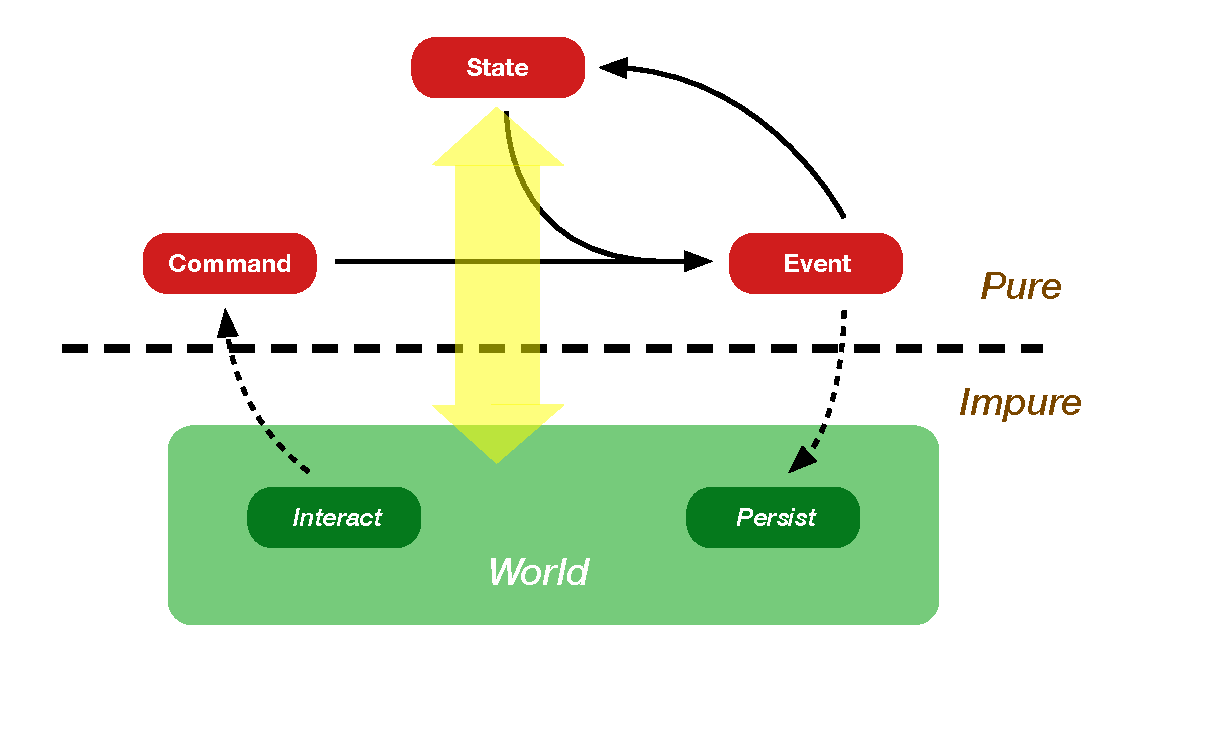
\includegraphics[width=\textwidth]{./images/event-loop.pdf}
\end{center}
\end{frame}

\begin{frame}[fragile]{Language}
  \begin{itemize}
  \item $C$ is the set of all Commands, $E$ the set of all Events, $S$ the set of states
  \item $$\delta : S \times C \times E^* \rightarrow S$$ a transition function between states $S$
  \item The language of a component $L \subseteq (C \times E^*)^*$ is a \textbf{transduction}
  \item We can simplify to $L \subseteq ((C + \epsilon) \times E)^*$
  \end{itemize}
\end{frame}

\begin{frame}[fragile]{Language}
  An \emph{Event Sourced} language is such that
  $$\forall s \in S, \exists t \in E^*, \exists c \in C^*, \delta(s_0,c \times t) = s $$
  e.g. the possible states of the system are determined by possible traces of events:
  $$S \subseteq E^*$$
\end{frame}

%%%%%%%%%%%%%%%%%%%%%%%%%%%%%%%%%%%%%%%%%%%%%%%%%%
\part{Homomorphic Event Sourcing}

\begin{frame}[fragile]{Interacting Components}
  \begin{itemize}
  \item What happens when 2 event-sourced components have to interact?
  \item We want to map commands $C_1$ must be mapped to commands $C_2$, and events $E_2$ to events $E_1$
  \end{itemize}
\end{frame}

\begin{frame}[fragile]{Base Event Loop}
\begin{center}
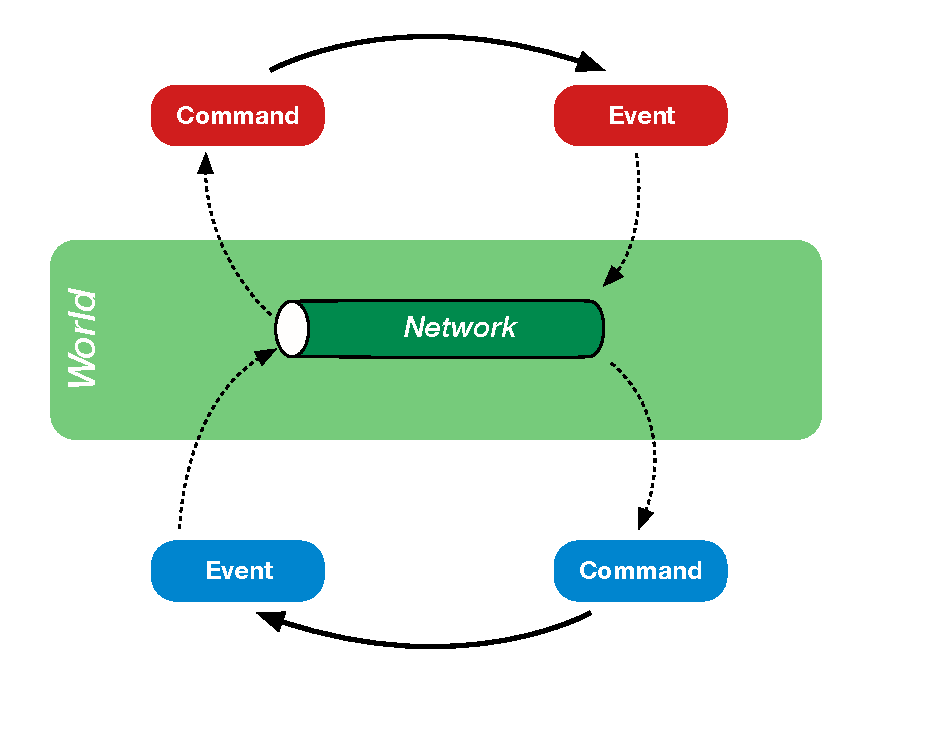
\includegraphics[height=.8\textheight]{./images/interaction-loop.pdf}
\end{center}
\end{frame}

\begin{frame}[fragile]{Homomorphism}

  A \emph{homomorphism} is a structure-preserving map between two languages. This practically means it is enough to
  define a \emph{map} from letters of one language to letters of the other

\end{frame}

\begin{frame}[fragile]{Homomorphic Event Sourcing}
  \begin{itemize}
  \item Define mappings from UI commands to backend commands: An event
    can map to nothing meaning there is not interaction with
    the backend
  \item Define mappings from backend events to UI events: Defines how
    backend's replies are interpreted in the UI
  \item Strive to define \emph{identities}, e.g. use the same language of commands and events in the frontend and the backendx
  \end{itemize}
\end{frame}

%%%%%%%%%%%%%%%%%%%%%%%%%%%%%%%%%%%%%%%%%%%%%%%%%%
\part{Consumer-Driven Contract Testing}

%%%%%%%%%%%%%%%%%%%%%%%%%%%%%%%%%%%%%%%%%%%%%%%%%%
\begin{frame}[fragile]{Standard Problem for Webapps?}

\begin{itemize}
\item Testing that frontend and backend play nicely together
\end{itemize}

\end{frame}

%%%%%%%%%%%%%%%%%%%%%%%%%%%%%%%%%%%%%%%%%%%%%%%%%%
\begin{frame}[fragile]{Standard Approach: ``Super-Na\"ive''}

\only<1>{
\begin{itemize}
\item Backend designs API
\item Backend is developed, tests are written
\item Frontend waits until backend is implemented
\item Frontend is developed
\item Tests for frontend are written
\item Interaction is tested via integration tests
\end{itemize}
}

\only<2>{
Problems:

\begin{itemize}
\item Frontend development is blocked
\item Integration tests are slow
\item Full integration testing does not scale
\end{itemize}
}

\end{frame}

%%%%%%%%%%%%%%%%%%%%%%%%%%%%%%%%%%%%%%%%%%%%%%%%%%
\begin{frame}[fragile]{Standard Approach: ``Still Quite Na\"ive''}

\only<1>{
\begin{itemize}
\item Backend designs API
\item Backend is developed, tests are written
\item Frontend writes mocks for backend API
\item Frontend can be developed immediately
\item Interaction tests for frontend use these mocks
\end{itemize}
}

\only<2>{
Problems:

\begin{itemize}
\item Frontend relies on mocks for backend API
\item Do the mocks reflect the backend's actual behaviour?
\item Usually, backend behaviour changes
\item Frontend does not notice because mocks still look good
\end{itemize}
}

\end{frame}

%%%%%%%%%%%%%%%%%%%%%%%%%%%%%%%%%%%%%%%%%%%%%%%%%%
\begin{frame}[fragile]{Standard ``Industry-Strength'' Approach}

\only<1>{
\begin{itemize}
\item Consumer-Driven Contract Testing
\item Hand-written contracts
\end{itemize}
}

\only<2>{
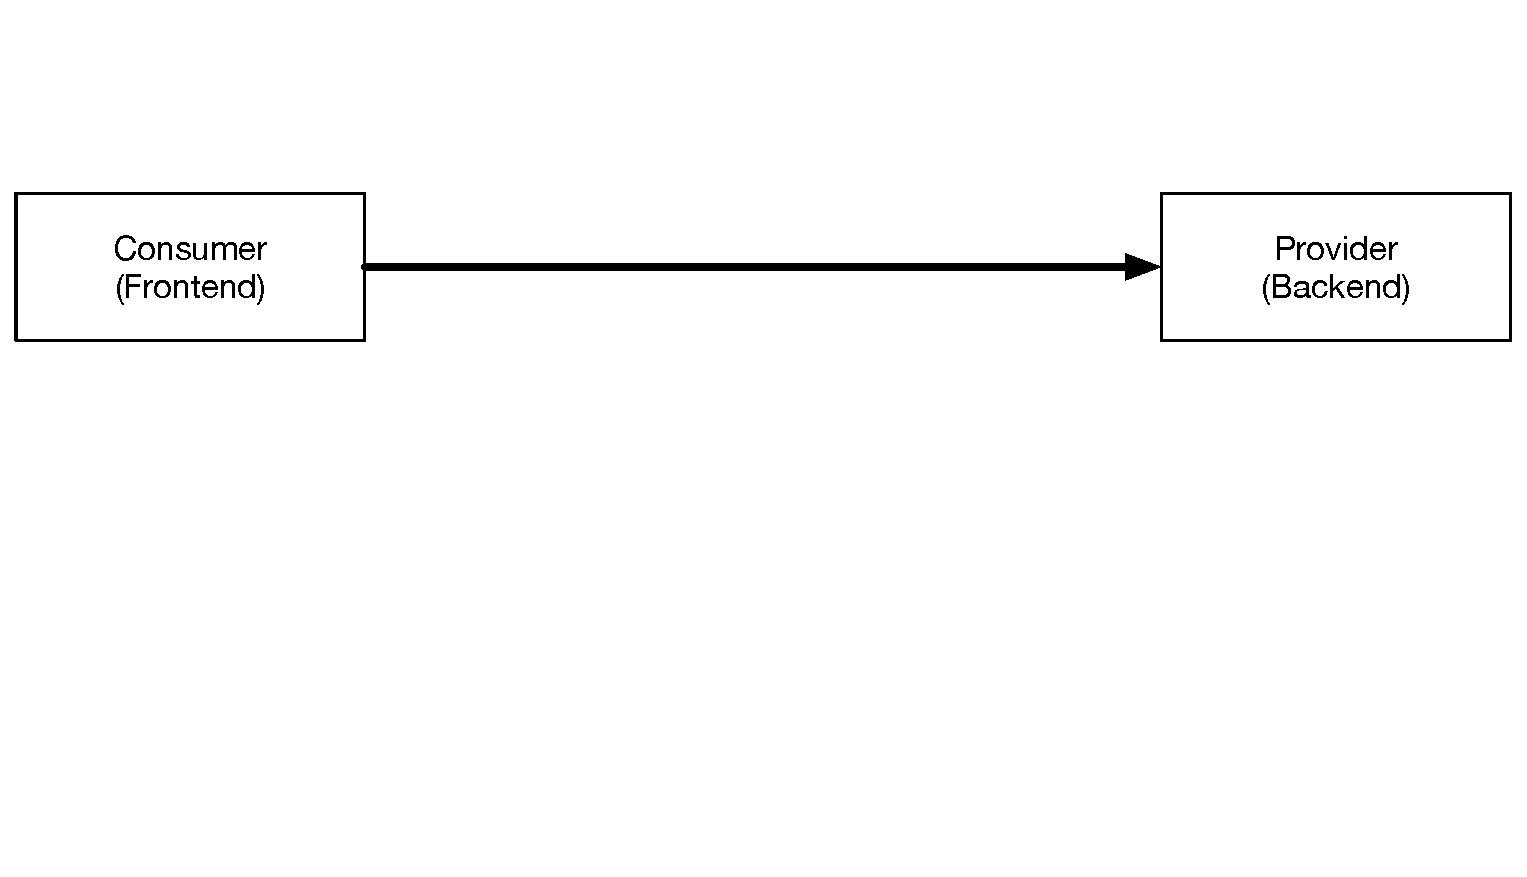
\includegraphics[width=\textwidth]{images/CDCT1.pdf}
}

\only<3>{
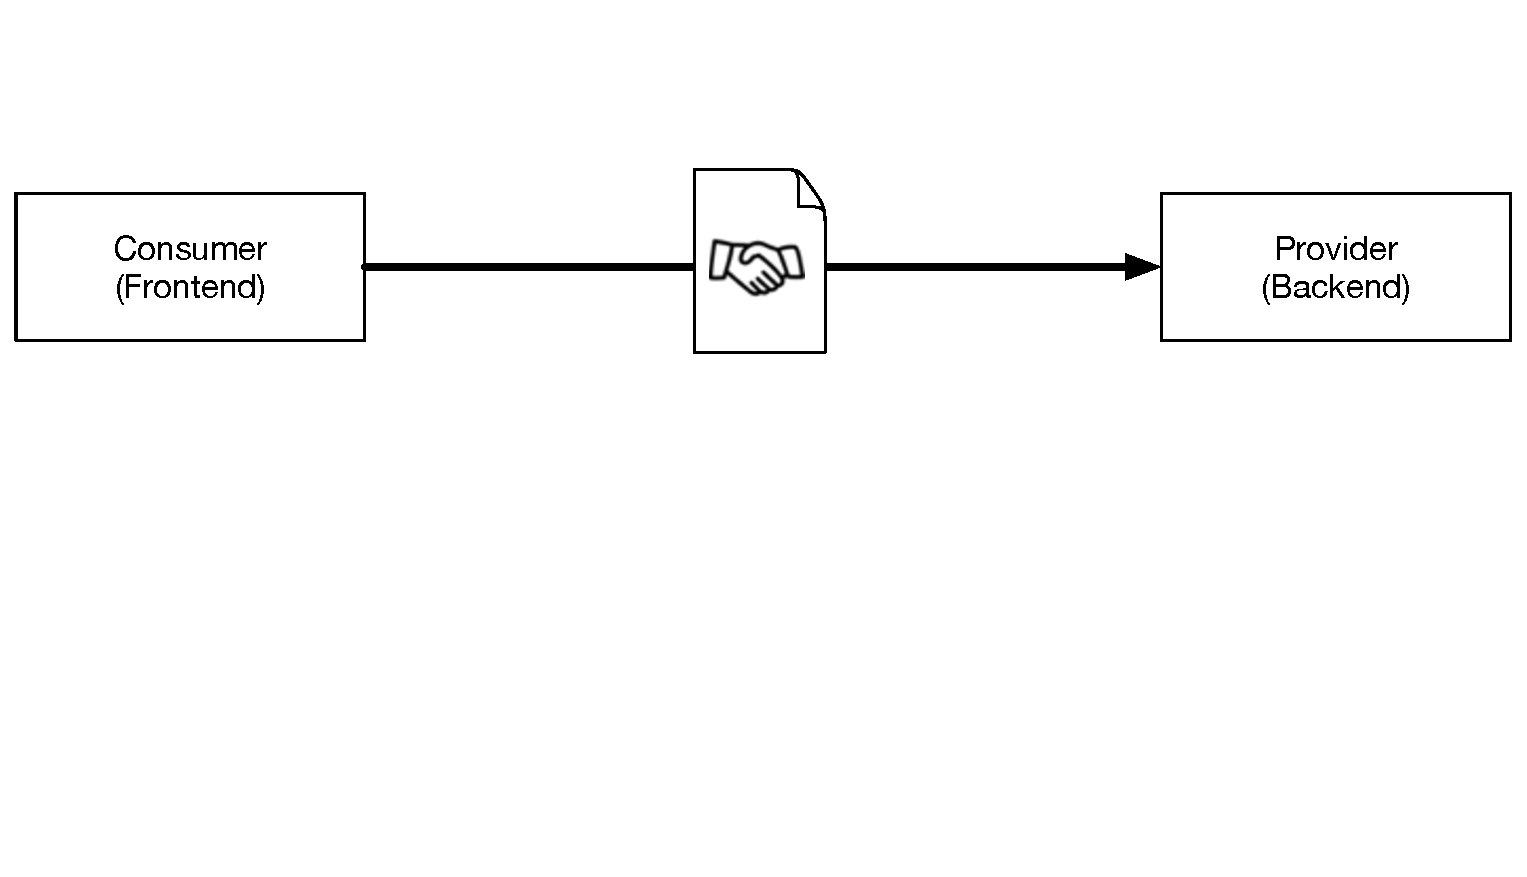
\includegraphics[width=\textwidth]{images/CDCT2.pdf}
}

\only<4>{
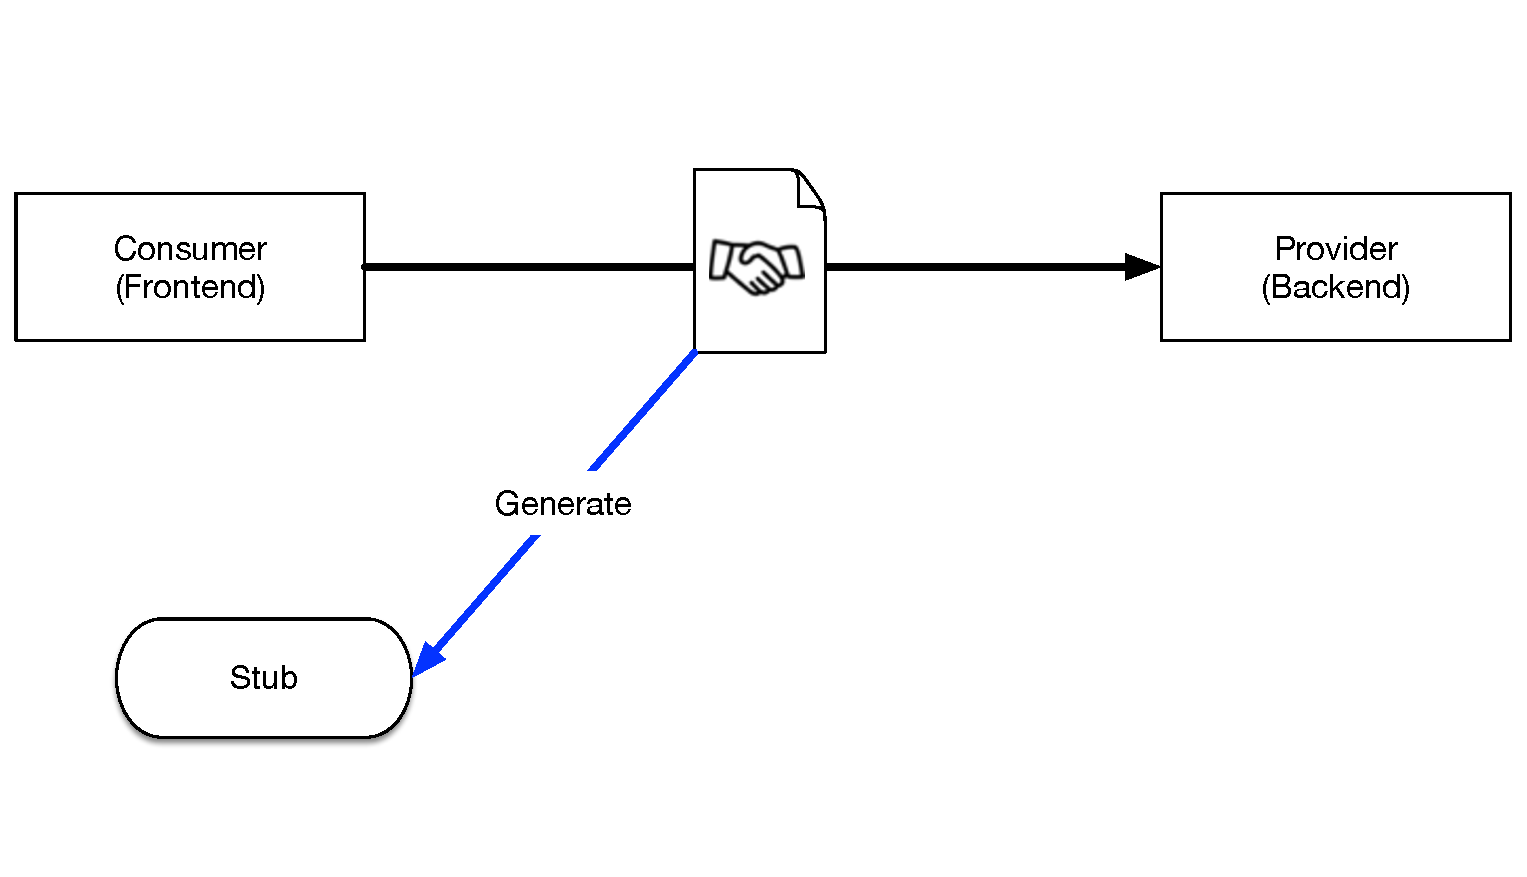
\includegraphics[width=\textwidth]{images/CDCT3.pdf}
}

\only<5>{
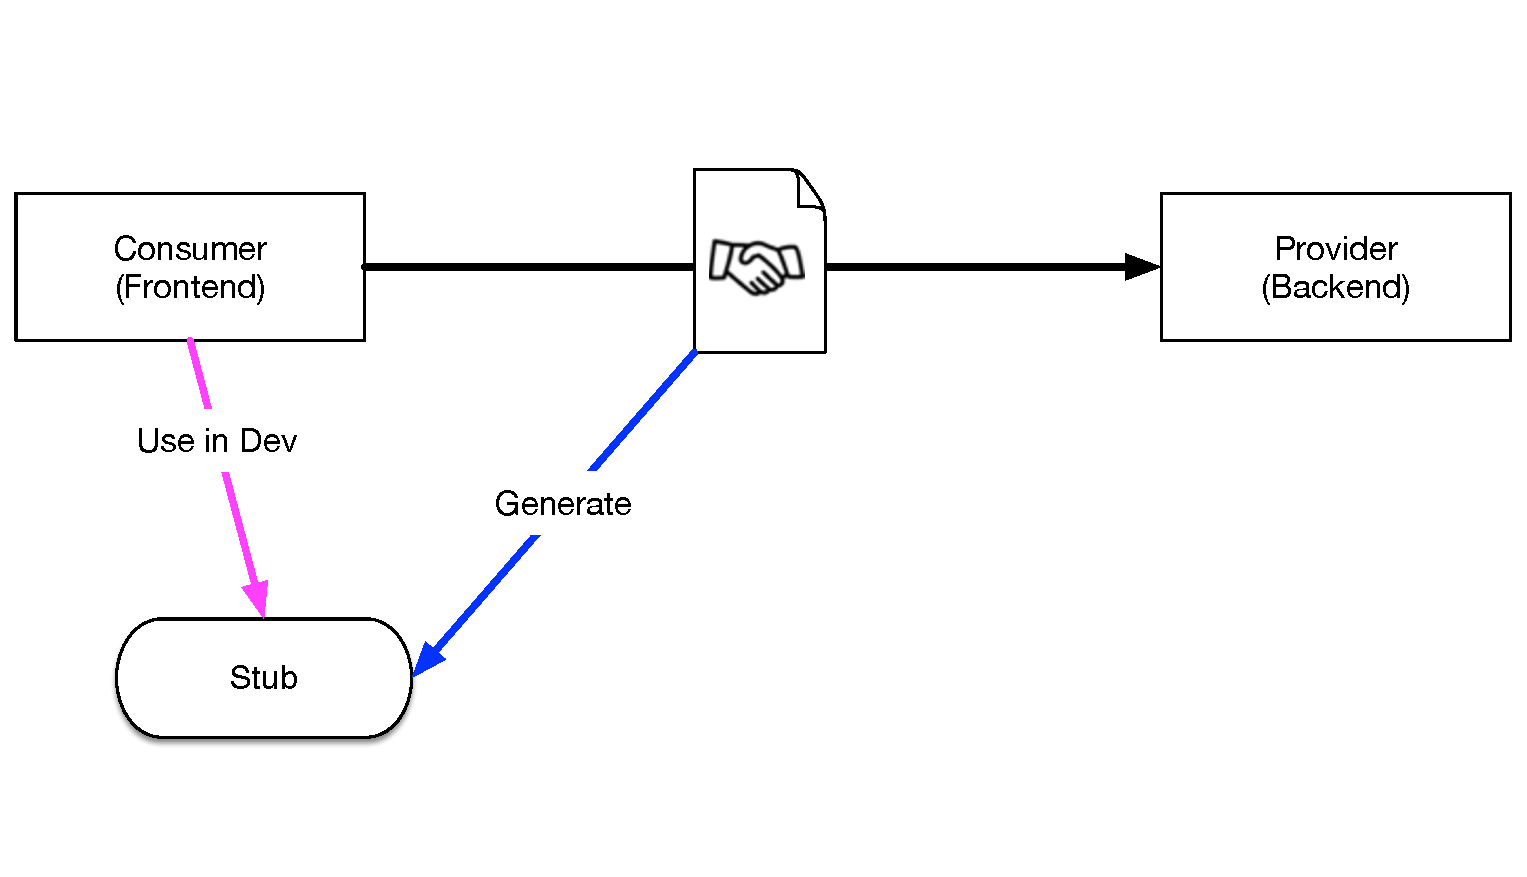
\includegraphics[width=\textwidth]{images/CDCT4.pdf}
}

\only<6>{
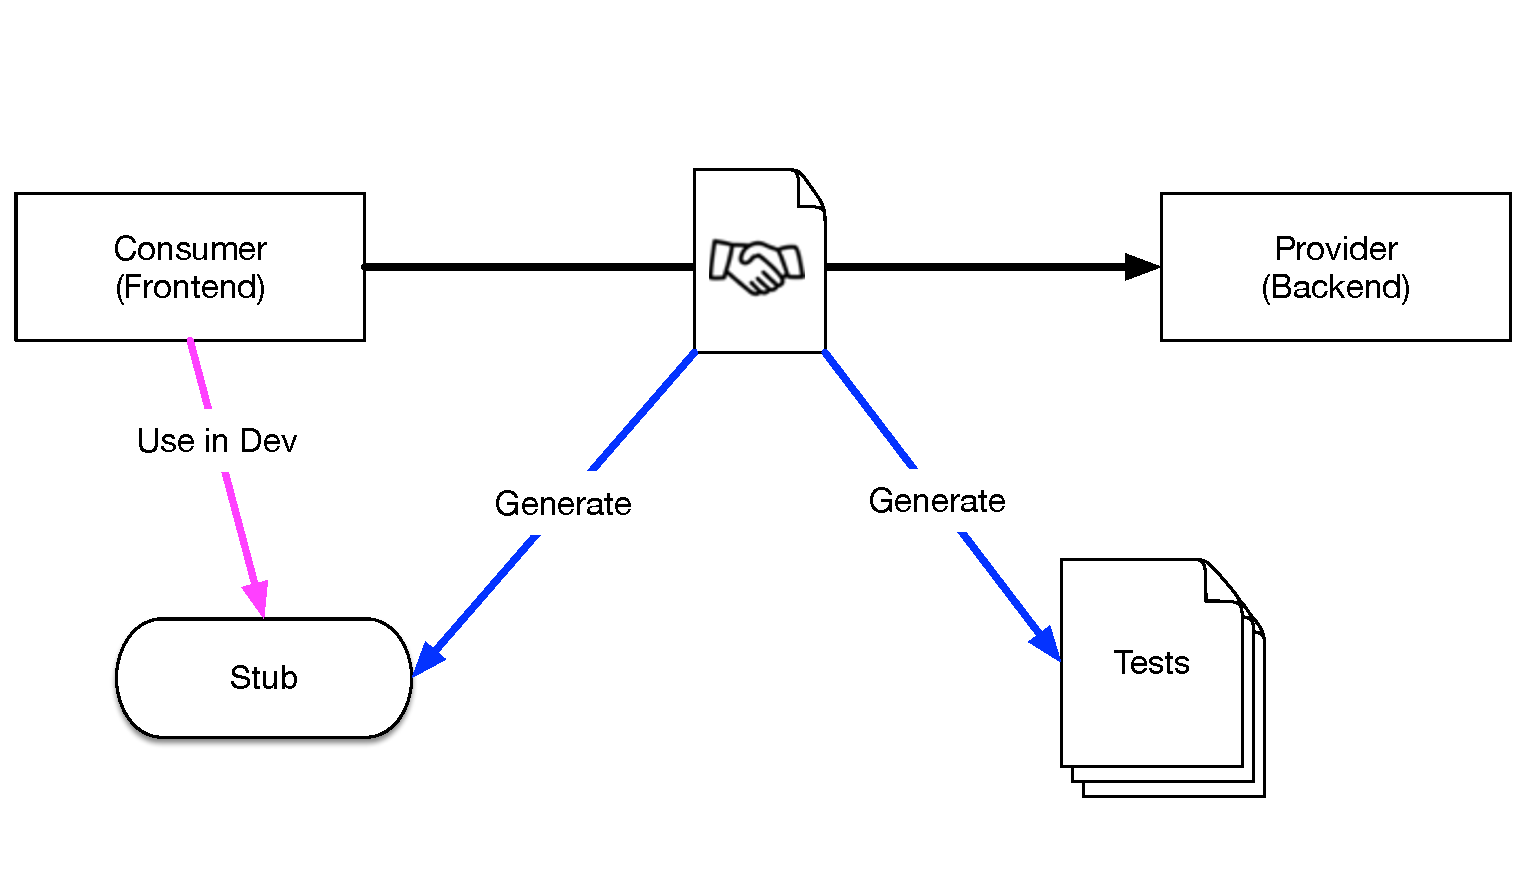
\includegraphics[width=\textwidth]{images/CDCT5.pdf}
}

\only<7>{
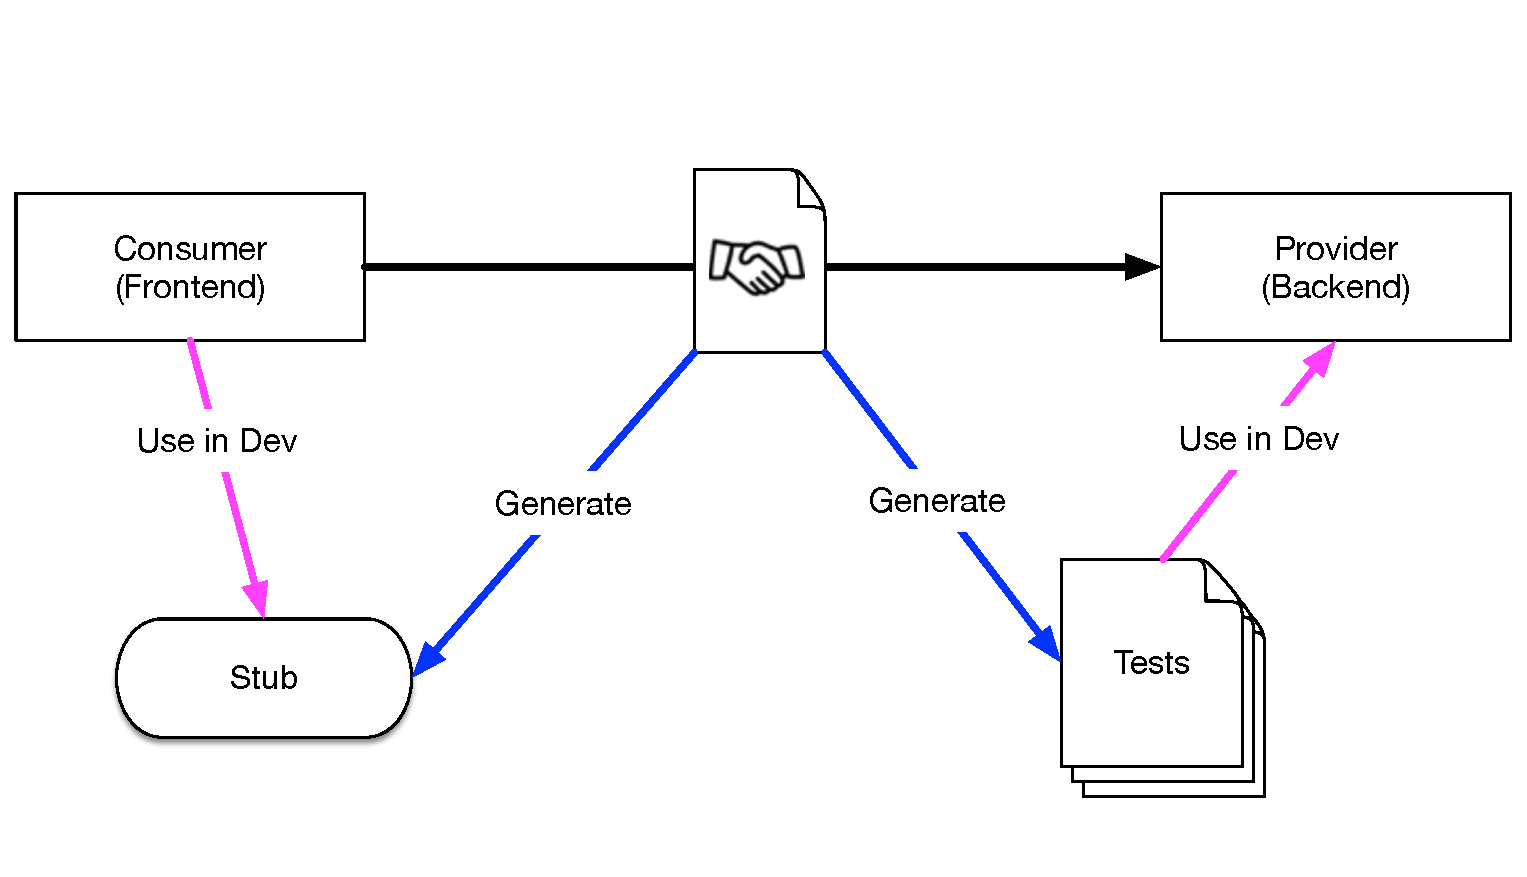
\includegraphics[width=\textwidth]{images/CDCT6.pdf}
}

\only<8>{
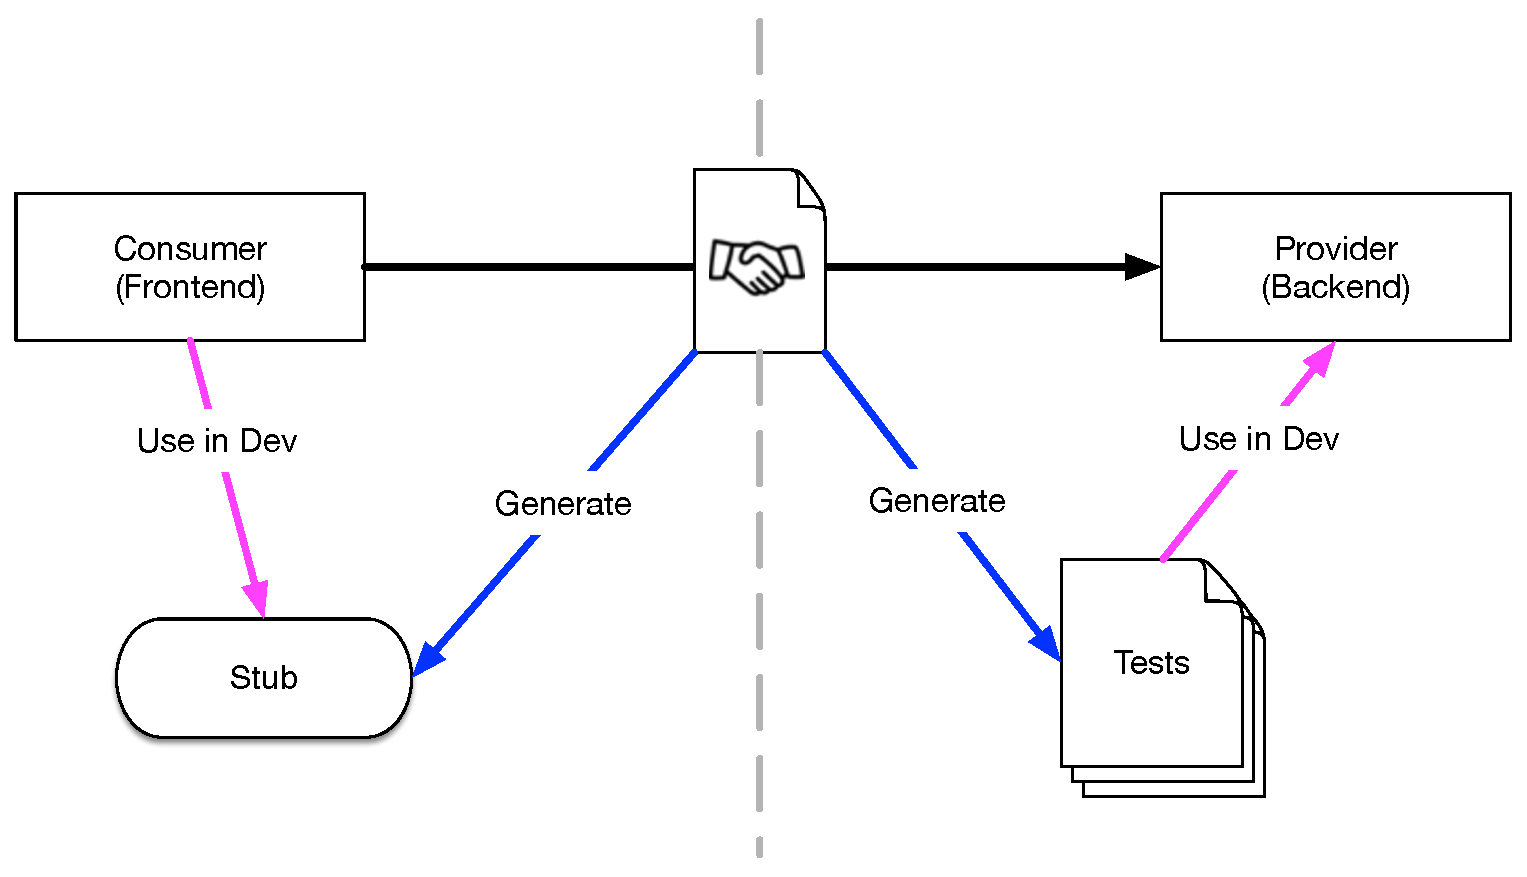
\includegraphics[width=\textwidth]{images/CDCT7.pdf}
}

\only<9>{
Problems:

\begin{itemize}
\item Contract testing is only as good as its contracts
\item Manual contract-writing can be tedious and even error-prone
\item Errors may only be discovered late in the process, when the backend implements some functionality and discovers that it does not match the contract
\item If contracts are too sparse, we miss out
\item If contracts are too verbose (or too many), testing takes too long
\end{itemize}
}

\end{frame}

\begin{frame}[fragile]{Beyond Homomorphism}
  \begin{itemize}
  \item Homomorphism do not account for \emph{current state}, e.g. what happened in the past
  \item Some events might be meaningfully interpreted only after some other events happened
  \item \emph{Homomorphism} $\longrightarrow$ \emph{Transduction}
  \end{itemize}
\end{frame}


\begin{frame}[fragile]{Our ``formal model'' approach}

\begin{enumerate}
\item Describe the Frontend-Backend integration in a formal model
\item Generate mocks for the frontend from this model
\item Generate tests for the backend from this model
\item Guarantee: All aspects (that are in the model) are covered by the tests and mocks
\end{enumerate}

\end{frame}
\begin{frame}[fragile]{Modelling with State Machines}
  \begin{itemize}
  \item Modelling the \emph{Code Domain}'s behaviour as a \emph{State Machine}
  \item Use the State Machine as a \emph{Generator} to test \emph{Backend}
  \item Use the State Machine as a \emph{Acceptor} to test \emph{Frontend}
  \end{itemize}
\end{frame}


%%%%%%%%%%%%%%%%%%%%%%%%%%%%%%%%%%%%%%%%%%%%%%%%%%
\part{Examples \& Demo}

\begin{frame}[fragile]{Acquire}
  \begin{center}
    
\includegraphics[height=.8\textheight]{./images/acquire-boardgame.jpg}
  \end{center}
\end{frame}

\begin{frame}[fragile]{Architecture - Backend}
  \begin{center}
    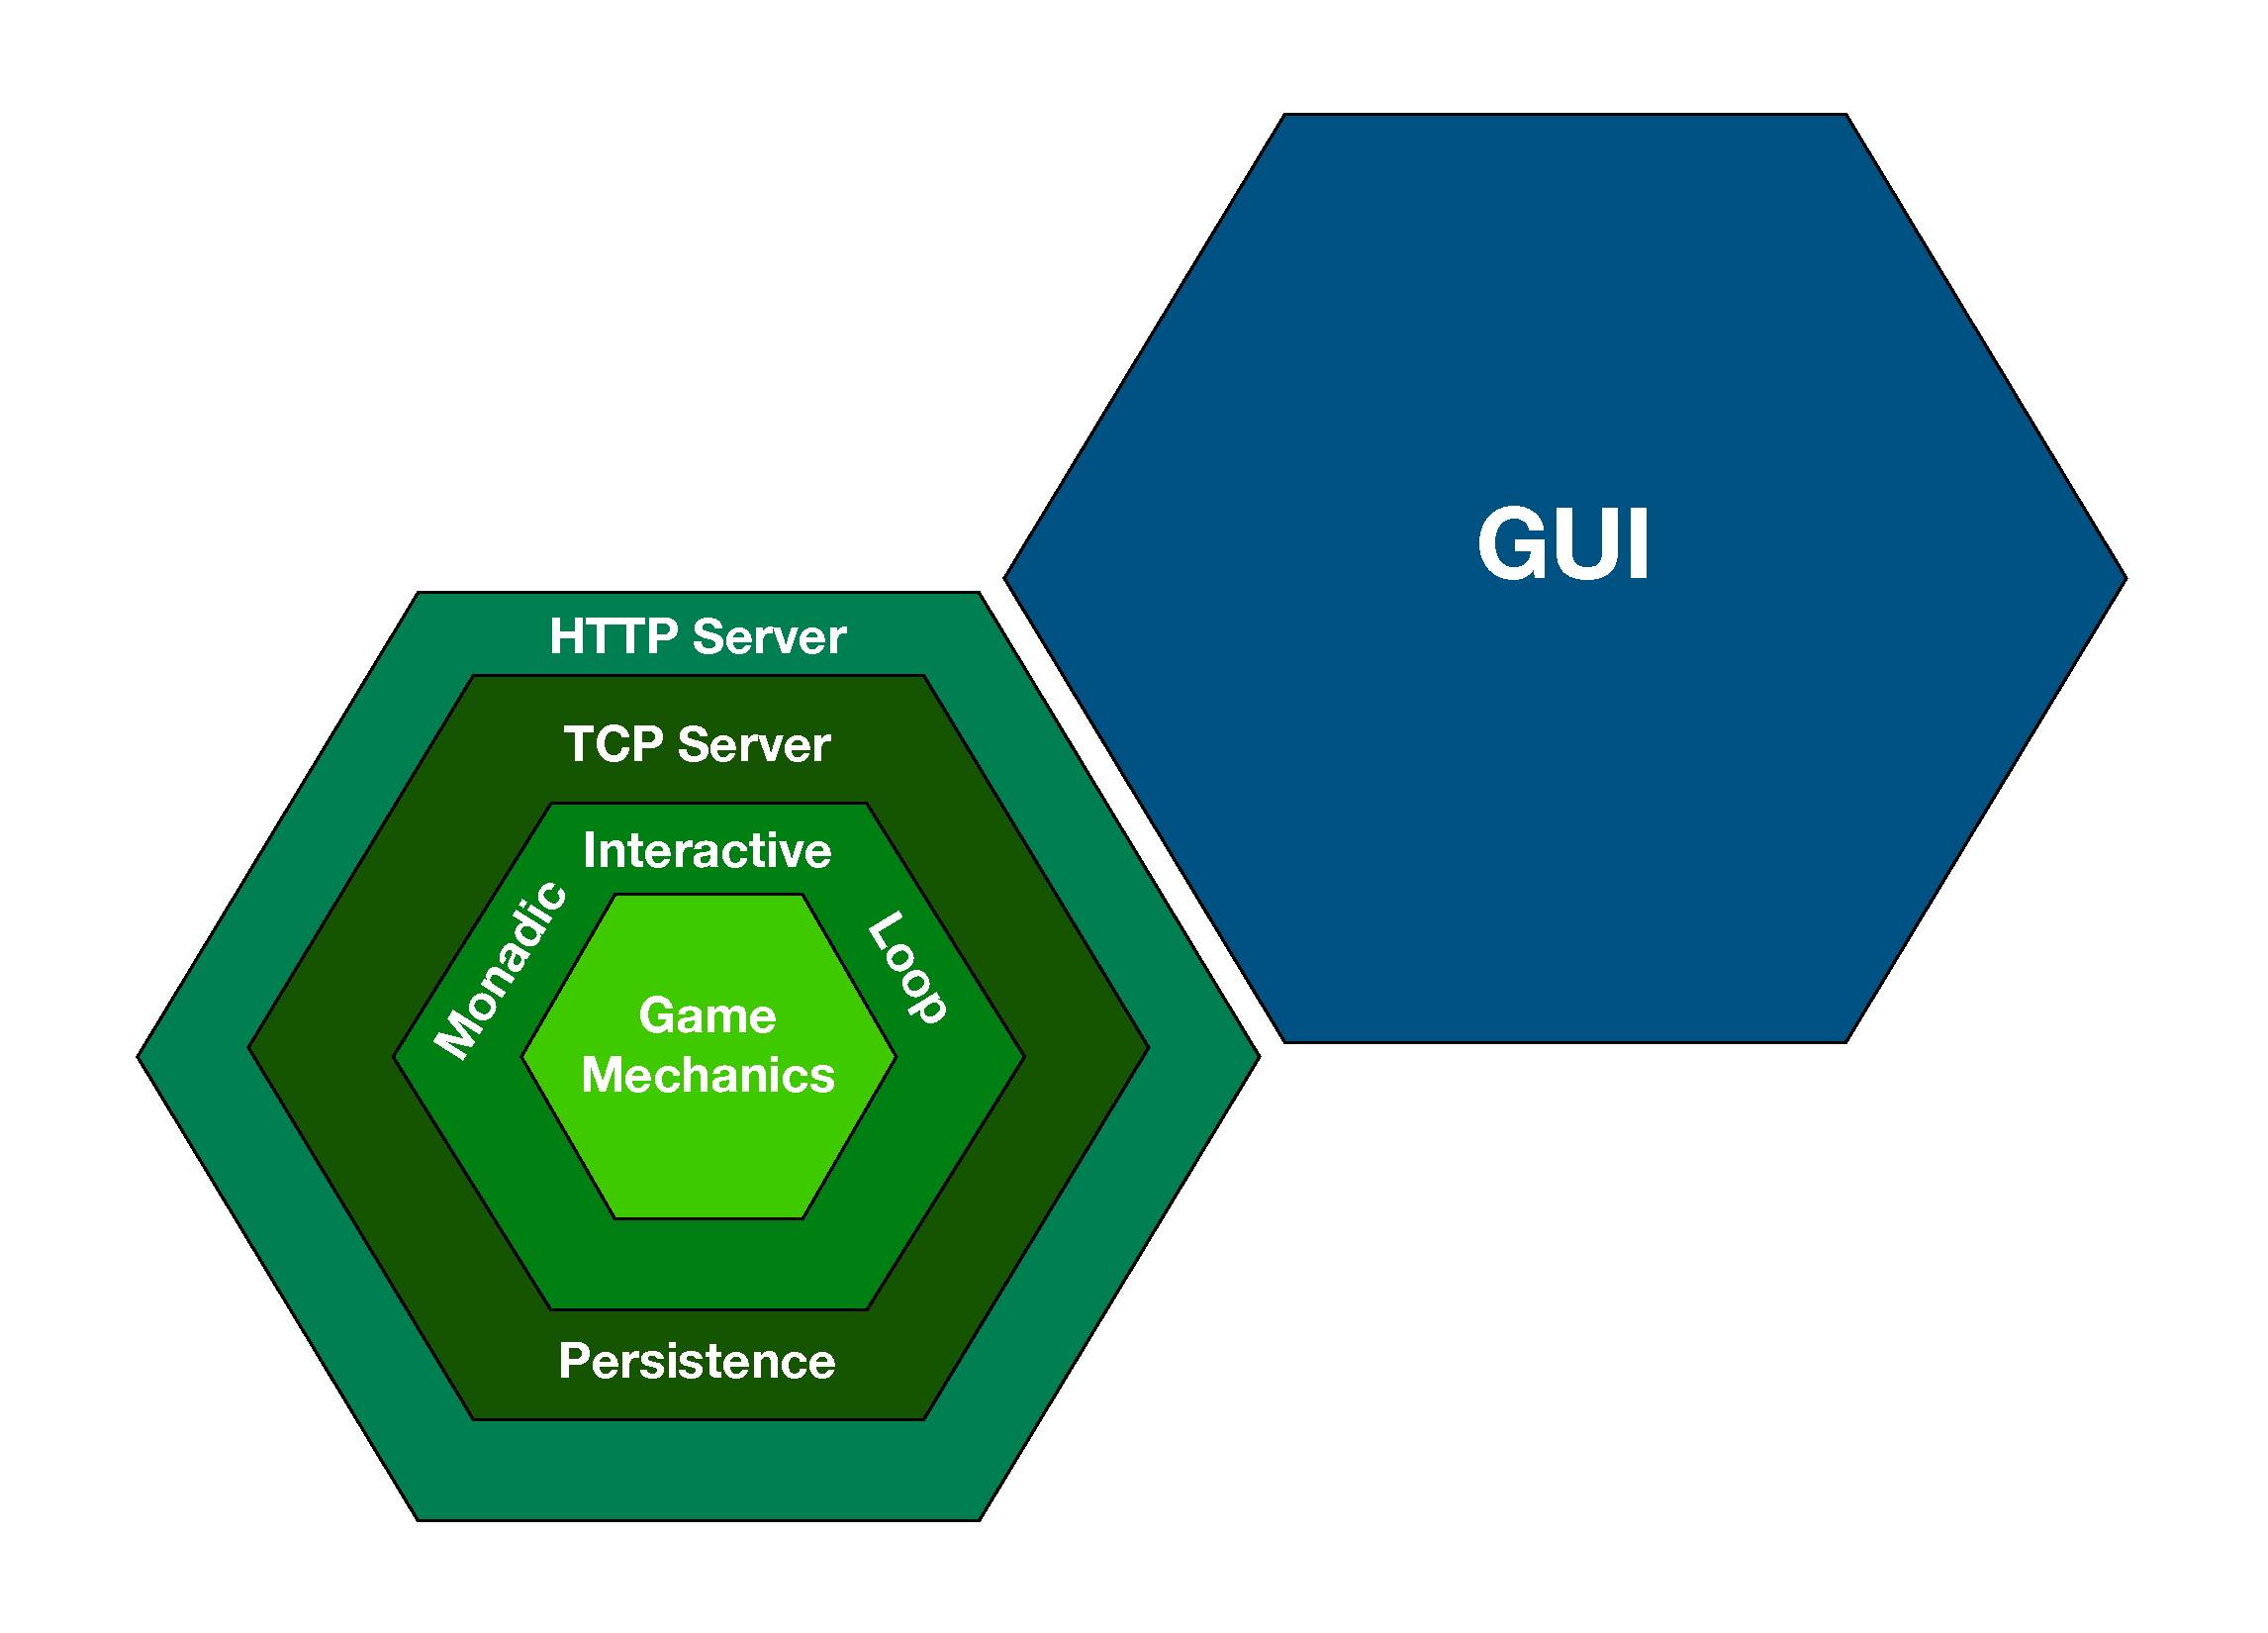
\includegraphics[height=.8\textheight]{./images/archi-back.pdf}
  \end{center}
\end{frame}

\begin{frame}[fragile]{Architecture - Frontend}
  \begin{center}
    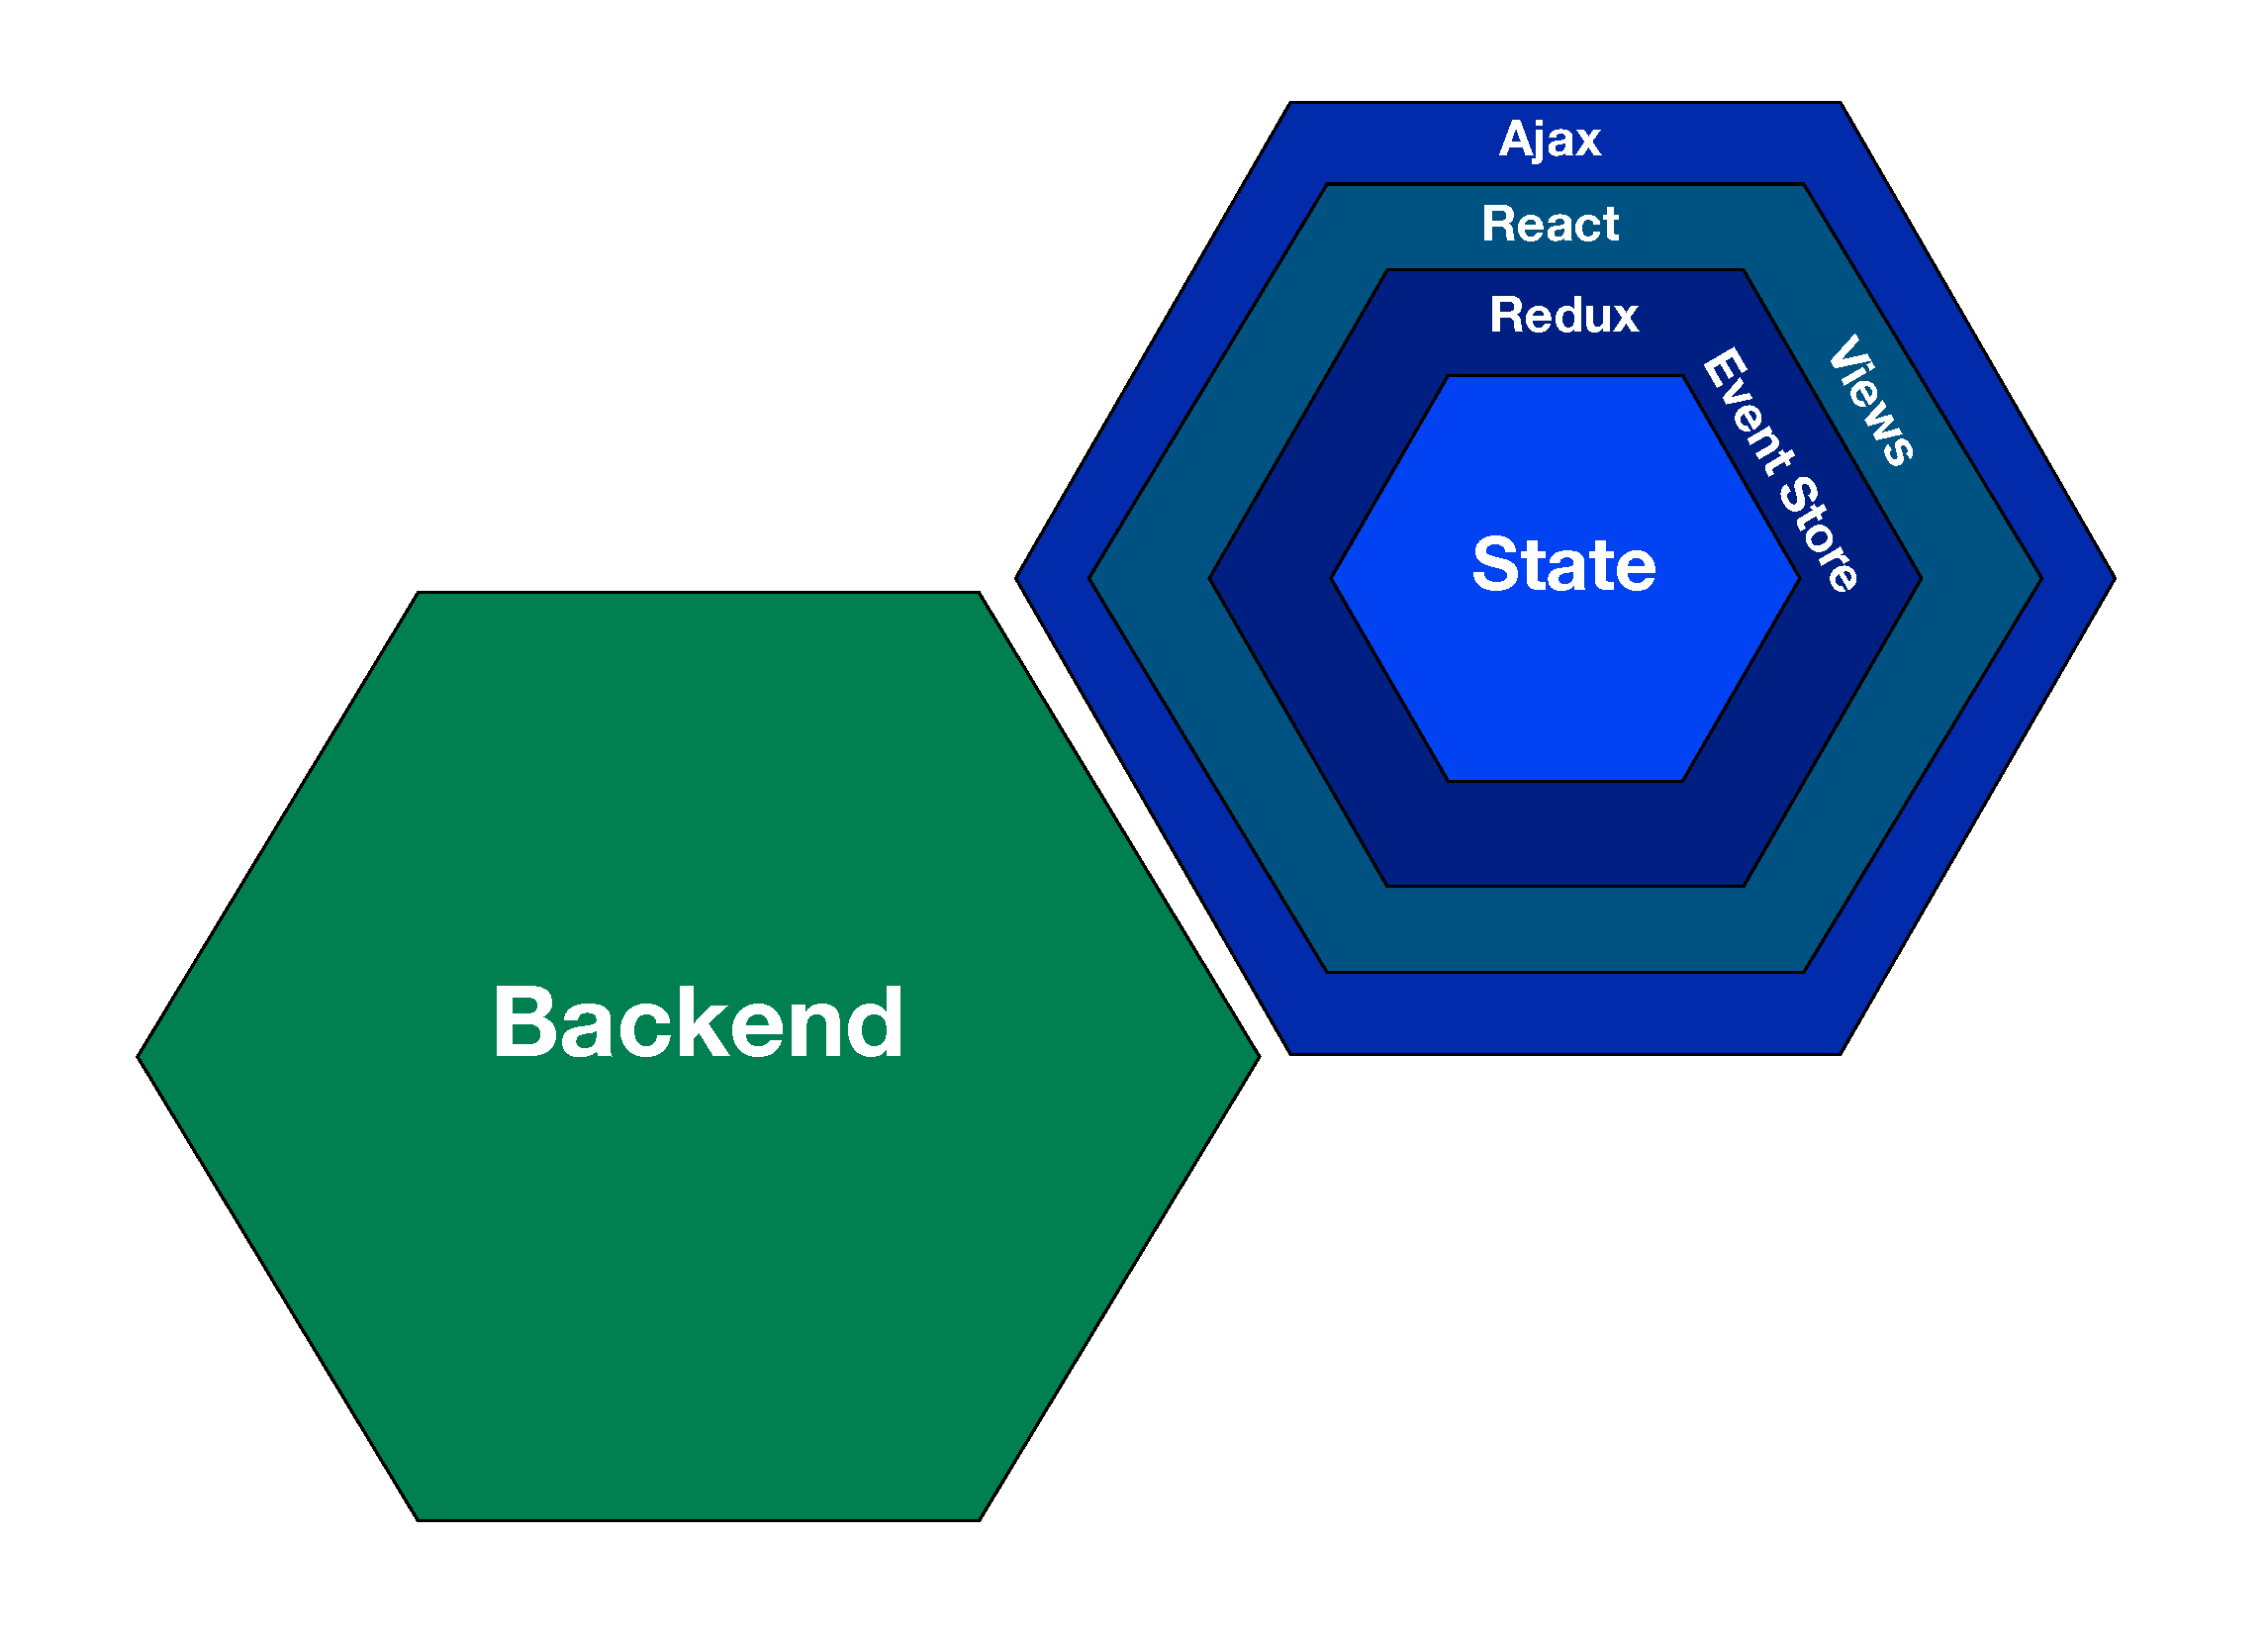
\includegraphics[height=.8\textheight]{./images/archi-front.pdf}
  \end{center}
\end{frame}

%%%%%%%%%%%%%%%%%%%%%%%%%%%%%%%%%%%%%%%%%%%%%%%%%%
\part{Conclusion}

\begin{frame}[fragile]{Takeaways}
  \only<1>{\Huge \begin{quote} Plans are worthless,\\ but planning is everything \\ \textsc{\Large Dwight D. Eisenhower}\end{quote}}
  \only<2>{\Huge \begin{quote} Models are worthless,\\ but modelling is everything \\ \textsc{\Large Nicole \& Arnaud}\end{quote}}
\end{frame}

\begin{frame}[fragile]{Event Sourcing $\leftrightarrow$ State Machines}
  \begin{itemize}[<+->]
  \item \emph{Event Sourcing} turns a system into an \emph{interpreter} for a language
  \item This makes it easy to model (part of) it as a \emph{State Machine}
  \end{itemize}
  \only<3>{\[
      \begin{array}{c}
        \text{Command} \times \text{State} \rightarrow \text{Event} \times \text{State} \\
         \Updownarrow \\
        \text{State} \xrightarrow{\text{Command} \times \text{Event}} \text{State} \\
      \end{array}
    \]}
\end{frame}

\begin{frame}[fragile]{Caveats}
  \begin{itemize}
  \item It takes time and energy to devise and refine a model
  \item It's not a \emph{Silver Bullet}\textsuperscript{\tiny TM}
  \end{itemize}
\end{frame}


%%%%%%%%%%%%%%%%%%%%%%%%%%%%%%%%%%%%%%%%%%%%%%%%%%
\begin{frame}{Thank you very much!}

  \url{https://github.com/}

  ~\\[1em]
  \begin{block}{Arnaud Bailly}
        \begin{description}[Twitterxx]
        \item[E-Mail]  \href{mailto:arnaud@aleryo.com}{\texttt{arnaud@aleryo.com}}
        \item[Twitter] \href{http://twitter.com/NicoleRauch}{\texttt{@dr\_c0d3}}
        \item[Web] \href{http://aleryo.com}{\texttt{http://aleryo.com}}
        \end{description}
  \end{block}
  \begin{block}{Nicole Rauch}
    \begin{description}[Twitterxx]
    \item[E-Mail]  \href{mailto:info@nicole-rauch.de}{\texttt{info@nicole-rauch.de}}
    \item[Twitter] \href{http://twitter.com/NicoleRauch}{\texttt{@NicoleRauch}}
    \item[Web] \href{http://www.nicole-rauch.de}{\texttt{http://www.nicole-rauch.de}}
    \end{description}
  \end{block}
\end{frame}

%% https://i2.wp.com/thebiggamehunter.com/wp-content/uploads/2011/02/Acquire-3M-Sid-Sackson-11.jpg
